%% ACO-TGFuse — Elsevier CAS double-column format (cas-dc)
\documentclass[a4paper,fleqn]{cas-dc}

\usepackage[numbers]{natbib}
\usepackage{cleveref}
\usepackage{subcaption}
\usepackage{float}
\usepackage{amssymb}
\usepackage{amsmath}
\usepackage{amsthm}
\newtheorem{proposition}{Proposition}[section]
\usepackage{graphicx}
\usepackage{multirow}
\usepackage{algorithm}
\usepackage{algpseudocode}
\usepackage{xcolor}
\usepackage{hyperref}
\usepackage{adjustbox}
\usepackage{booktabs}
\usepackage{array}
\usepackage{stfloats}   % allows figure* to use [b] and [h] in two-column
\usepackage{placeins}   % provides \FloatBarrier

\begin{document}
\let\WriteBookmarks\relax
\def\floatpagepagefraction{1}
\def\textpagefraction{.001}

\shorttitle{ACO-TGFuse: Ant Colony Optimization-Guided Transformer Fusion for IVIF}

\title[mode=title]{ACO-TGFuse: Ant Colony Optimization-Guided Transformer Fusion for Infrared and Visible Image Fusion}

\author[1]{Duc Cuong Pham}

\address[1]{Faculty of Information Technology, [Institution], Vietnam}

\begin{abstract}
Infrared and visible image fusion (IVIF) aims to produce a composite image
that combines the thermal saliency of infrared with the structural richness
of visible light.  Existing deep learning methods rely on manually designed
fusion architectures in which the selection of encoder scales for cross-modal
interaction is largely unexplored.  We propose ACO-TGFuse, a framework that
integrates Ant Colony Optimization (ACO) as a one-time offline architecture
search over all six pairwise combinations of a four-level multi-scale encoder,
identifying the most complementary scale pair without any inference overhead.
The search converges to the ($\mathrm{en}_0$, $\mathrm{en}_3$) pair, bridging
fine-grained texture features with coarse-level thermal structure.  A
Cross-modal Relation Map derived by sequential Channel and Spatial Transformers
is broadcast to four encoder scales, yielding Relation-guided Multi-scale
Fusion Masks $M_0$--$M_3$.  A Cross-Branch Attention module further refines
interaction between the two ACO-selected branches, and dual-discriminator
adversarial training sharpens visual fidelity.  Evaluated on TNO, RoadScene,
and MSRS, ACO-TGFuse achieves the highest SSIMv and $Q_{abf}$ scores on all
three datasets, with competitive performance across eight standard metrics.
\end{abstract}

\begin{highlights}
\item Offline ACO search over all $\binom{4}{2}=6$ encoder branch pairs
      identifies the optimal ($\mathrm{en}_0$+$\mathrm{en}_3$) configuration
      with no inference overhead.

\item A Cross-modal Relation Map (1-channel) derived from sequential Channel
      and Spatial Transformers is broadcast to four scales, guiding
      Relation-guided Multi-scale Fusion Masks $M_0$--$M_3$.

\item Cross-Branch Attention enables bidirectional feature interaction between
      the fine-resolution and coarse-resolution ACO-selected branches.

\item ACO-TGFuse achieves the best SSIMv and $Q_{abf}$ on TNO, RoadScene, and
      MSRS benchmarks simultaneously.
\end{highlights}

\begin{keywords}
Infrared and visible image fusion \sep
Neural architecture search \sep
Ant colony optimization \sep
Transformer attention \sep
Multi-scale feature fusion
\end{keywords}

\maketitle

%% ════════════════════════════════════════════════════════════════
\section{Introduction}
\label{sec:intro}
%% ════════════════════════════════════════════════════════════════

Infrared (IR) and visible (VIS) imaging are complementary sensing modalities
whose individual limitations motivate their joint use.  Infrared sensors
capture thermal radiation emitted by objects, enabling detection of pedestrians
and vehicles in complete darkness, fog, or smoke, but they lack color, fine
texture, and high spatial resolution.  Visible cameras record reflected ambient
light, providing rich structural detail and colour, but fail under low
illumination or high-contrast scenes.  Infrared and visible image fusion
(IVIF) combines both modalities into a single image that preserves the
thermal saliency of IR while retaining the structural richness of
VIS~\cite{u2fusion2022,piafusion2022,tardal2022}.  The resulting composite
enhances the performance of downstream perception tasks such as object
detection, semantic segmentation, and autonomous driving, which motivates
growing research interest in IVIF as a pre-processing stage for multi-sensor
perception pipelines.

Deep learning has substantially advanced IVIF over the past
decade~\cite{densefuse2019,swinfusion2022,cddfuse2023,emma2024}.
Autoencoder-based methods such as DenseFuse~\cite{densefuse2019} and
U2Fusion~\cite{u2fusion2022} learn shared feature representations through
encoder--decoder architectures, using hand-crafted rules ($\ell_1$-norm,
softmax weighting) for feature fusion.  GAN-based
approaches~\cite{gan2014,tgfuse2023} introduce adversarial training to
preserve source statistics, achieving sharper textures at the cost of
training instability.  Transformer-based methods have recently become
dominant: SwinFusion~\cite{swinfusion2022} exploits Swin Transformer blocks
for cross-domain long-range dependencies; CDDFuse~\cite{cddfuse2023}
decomposes features into base and detail components via dual-branch
correlation; EMMA~\cite{emma2024} adopts a visual modality masking adapter to
bridge heterogeneous modalities.  TGFuse~\cite{tgfuse2023} combines
Transformer global modelling with GAN adversarial training, providing the
direct architectural foundation for this work.  Despite their strengths,
all of these methods rely on manually designed fusion architectures in which
hyperparameters such as the number of encoder stages and feature dimensions
are set by human intuition.

Three important design questions remain inadequately addressed in the
literature.  First, \emph{which encoder scales should be coupled for
cross-modal interaction?}  Multi-scale feature hierarchies encode different
semantic and spatial information, yet no prior work systematically studies
which pair of scales is most complementary for IVIF; existing methods either
fuse all scales with equal weight or select arbitrarily.  Second,
\emph{how should cross-modal relational context be propagated across scales?}
Transformers typically compute attention at a single resolution, limiting
their ability to simultaneously model fine-grained texture alignment and
coarse thermal structure.  Propagating a compact single-channel relation map
to multiple scales could provide lightweight yet effective guidance, but this
design has not been explored.  Third, \emph{how should multi-scale features
be aggregated adaptively?}  Uniform summation ignores the fact that different
scenes may benefit from different scale emphases (e.g., thermally dominated
scenes vs.\ detail-rich scenes), suggesting that content-adaptive aggregation
is preferable.

To address these gaps, we propose \textbf{ACO-TGFuse}, which makes the
following contributions.  (i)~We introduce an \emph{offline} ACO-based neural
architecture search that evaluates all $\binom{4}{2}=6$ encoder branch pairs
and identifies the configuration ($\mathrm{en}_0$+$\mathrm{en}_3$) that
maximises a validation reward without any inference overhead---the search is
conducted once and the selected pair is fixed thereafter.  The importance of
the ACO formulation lies in its principled pheromone-based exploration: a
scale-distance heuristic biases the search towards complementary receptive
fields, while pheromone reinforcement focuses subsequent evaluations on
empirically strong configurations.  This automated selection replaces
the error-prone human trial-and-error that underlies existing methods.
(ii)~We design a \emph{Cross-modal Relation Map} module that applies
sequential Channel and Spatial Transformers to produce a single-channel map
at the deepest encoder scale, then resizes and broadcasts it to four
encoder levels to generate \emph{Relation-guided Multi-scale Fusion Masks}
$M_0$--$M_3$.  (iii)~We propose \emph{Cross-Branch Attention} between the
two ACO-selected branches to enable bidirectional, scale-aware cross-modal
interaction.  (iv)~Extensive evaluation on TNO, RoadScene, and MSRS
demonstrates that ACO-TGFuse achieves the best SSIMv and $Q_{abf}$ on all
three benchmarks simultaneously, with competitive performance across eight
standard metrics.

%% ════════════════════════════════════════════════════════════════
\section{Related Work}
\label{sec:related}
%% ════════════════════════════════════════════════════════════════

\subsection{Infrared and visible image fusion}
\label{sec:rw:ivif}

IVIF methods fall broadly into traditional and deep learning categories.
Traditional approaches --- including multi-scale transform
methods~\cite{tno2014}, sparse representation, and subspace decomposition
--- rely on hand-crafted priors for both feature extraction and fusion rule
design.  While interpretable, their fixed rules cannot adapt to scene
diversity and fail to capture cross-modal semantic correlations.

Among deep learning approaches, \emph{autoencoder-based} methods learn
intermediate representations that encode salient features from both
modalities.  DenseFuse~\cite{densefuse2019} introduces dense connectivity
in the encoder to preserve multi-scale features, using $\ell_1$-norm or
softmax fusion.  U2Fusion~\cite{u2fusion2022} unifies multiple fusion tasks
under a single framework with a unified unsupervised loss that measures
information preservation from each source.  RFNet~\cite{rfnet2023} jointly
addresses image registration and fusion in a mutually reinforcing framework.
While these methods avoid adversarial instability, their hand-crafted fusion
rules limit flexibility.

\emph{GAN-based} methods~\cite{gan2014} introduce adversarial objectives to
enforce that the fused image is statistically consistent with each source
modality.  TGFuse~\cite{tgfuse2023} employs Transformer encoders with a
dual-discriminator GAN to simultaneously preserve infrared saliency and
visible texture detail.  PIAFusion~\cite{piafusion2022} adds
illumination-aware progressive training: an illumination-aware sub-network
modulates the fusion strategy between day and night scenes.
TarDAL~\cite{tardal2022} jointly optimises IVIF and downstream object
detection through a target-aware dual adversarial learning strategy.
GAN training can produce visually sharp results but is notoriously
sensitive to hyperparameter settings and mode collapse.

\emph{Transformer-based} methods have become dominant for their ability to
model long-range dependencies.  SwinFusion~\cite{swinfusion2022} employs
Swin Transformer blocks with cross-domain attention that alternates between
intra-domain self-attention and inter-domain cross-attention to couple
IR and VIS features across the full spatial extent.  CDDFuse~\cite{cddfuse2023}
proposes a correlation-driven dual-branch architecture: a base encoder captures
low-frequency shared features, while a detail encoder handles
modality-specific high-frequency components, with inter-modality interaction
driven by pairwise feature correlation.  EMMA~\cite{emma2024} introduces a
visual modality masking adapter that efficiently adapts a pretrained vision
foundation model to the fusion task by masking and reconstructing modality-
specific tokens.  Despite strong results, these methods share a common
limitation: the coupling topology (which encoder stages interact and at what
scale) is fixed by manual design, with no principled study of which scale
combination is most informative.

\subsection{Neural architecture search}
\label{sec:rw:nas}

Neural Architecture Search (NAS)~\cite{nas2019} automates network design by
searching over a predefined architecture space.  Early reinforcement
learning-based approaches~\cite{nas2019} achieved strong results but required
thousands of GPU-hours.  Gradient-based methods such as
DARTS~\cite{oneshotnas2020} relax the discrete search into a differentiable
continuous relaxation, enabling efficient joint optimisation of architecture
and weights.  One-shot NAS methods~\cite{oneshotnas2020} train a single
supernet and derive candidate architectures by weight sharing, further
reducing search cost.

Swarm-intelligence methods offer a complementary perspective.  Ant Colony
Optimisation (ACO)~\cite{aco1992} was originally formulated for combinatorial
optimisation on graphs: artificial ants deposit pheromone on edges
proportional to solution quality, and subsequent ants preferentially follow
high-pheromone paths.  This mechanism provides a natural balance between
exploitation of strong solutions and exploration of alternatives.  In the
context of ACO-TGFuse, the search space consists of only $\binom{4}{2}=6$
branch pair candidates, making ACO highly efficient: each ant evaluates one
candidate architecture on a short training episode, and the pheromone
accumulation directs subsequent rounds towards the most promising
configurations.  Unlike DARTS, which requires maintaining a continuous weight
over all operations throughout training, ACO evaluates architectures
independently and converges in a small number of rounds.  Crucially, the
entire ACO search is conducted \emph{before deployment}; at inference, the
network runs as a fixed, standard architecture with no additional cost.

\subsection{Transformer attention in image fusion}
\label{sec:rw:transformer}

Self-attention and cross-attention mechanisms from the Transformer
architecture~\cite{t2tvit2021} have been widely applied to image fusion.
\emph{Channel attention} re-weights feature channels to suppress redundant
activations; \emph{spatial attention} identifies discriminative pixel
locations.  Applied to IVIF, channel attention can identify which channels
encode thermal structure vs.\ texture detail, while spatial attention
localises salient targets (hot pedestrians, structured edges).

The Token-to-Token Vision Transformer~\cite{t2tvit2021} progressively
restructures spatial tokens to capture both local fine-grained structure and
global context, motivating our use of the same mechanism for the Cross-modal
Relation Map.  Specifically, we apply a Channel Transformer followed by a
Spatial Transformer, both operating on the deepest encoder feature map
($32{\times}32$), to generate a single-channel relation map that summarises
cross-modal co-activation.  By compressing the representation to one channel,
the map captures cross-modal contrast without entangling it with
per-channel feature statistics, providing a lightweight guidance signal
that can be broadcast to all encoder scales.

Distinct from methods that apply full Transformer blocks at every
scale~\cite{swinfusion2022}, our approach computes the relation map once
and upsample-broadcasts it, substantially reducing parameter count and FLOPs
at higher encoder resolutions while still enabling multi-scale guidance.

\subsection{Multi-scale feature fusion}
\label{sec:rw:multiscale}

Feature pyramid networks~\cite{vgg2015} demonstrated that fusing features
across multiple spatial resolutions substantially improves detection and
segmentation.  In IVIF, multi-scale representations allow simultaneous
preservation of fine texture (high-resolution features) and semantic thermal
context (low-resolution features).  Existing fusion methods typically merge
all scales through summation or concatenation with learnable weights.

A critical and understudied question is \emph{which scale pairs are most
complementary} for the specific cross-modal alignment problem in IVIF.
Intuitively, pairing the finest resolution (rich in texture edges) with the
coarsest resolution (rich in semantic thermal regions) should maximise
complementarity.  ACO-TGFuse empirically validates this intuition through
systematic search, finding that $(\mathrm{en}_0, \mathrm{en}_3)$ achieves
the highest SF and EN among all six candidates, confirming that maximal
scale distance in the encoder hierarchy is a reliable heuristic for
complementarity.

%% ════════════════════════════════════════════════════════════════
\section{Proposed Method}
\label{sec:method}
%% ════════════════════════════════════════════════════════════════

\begin{figure*}[!ht]
  \centering
  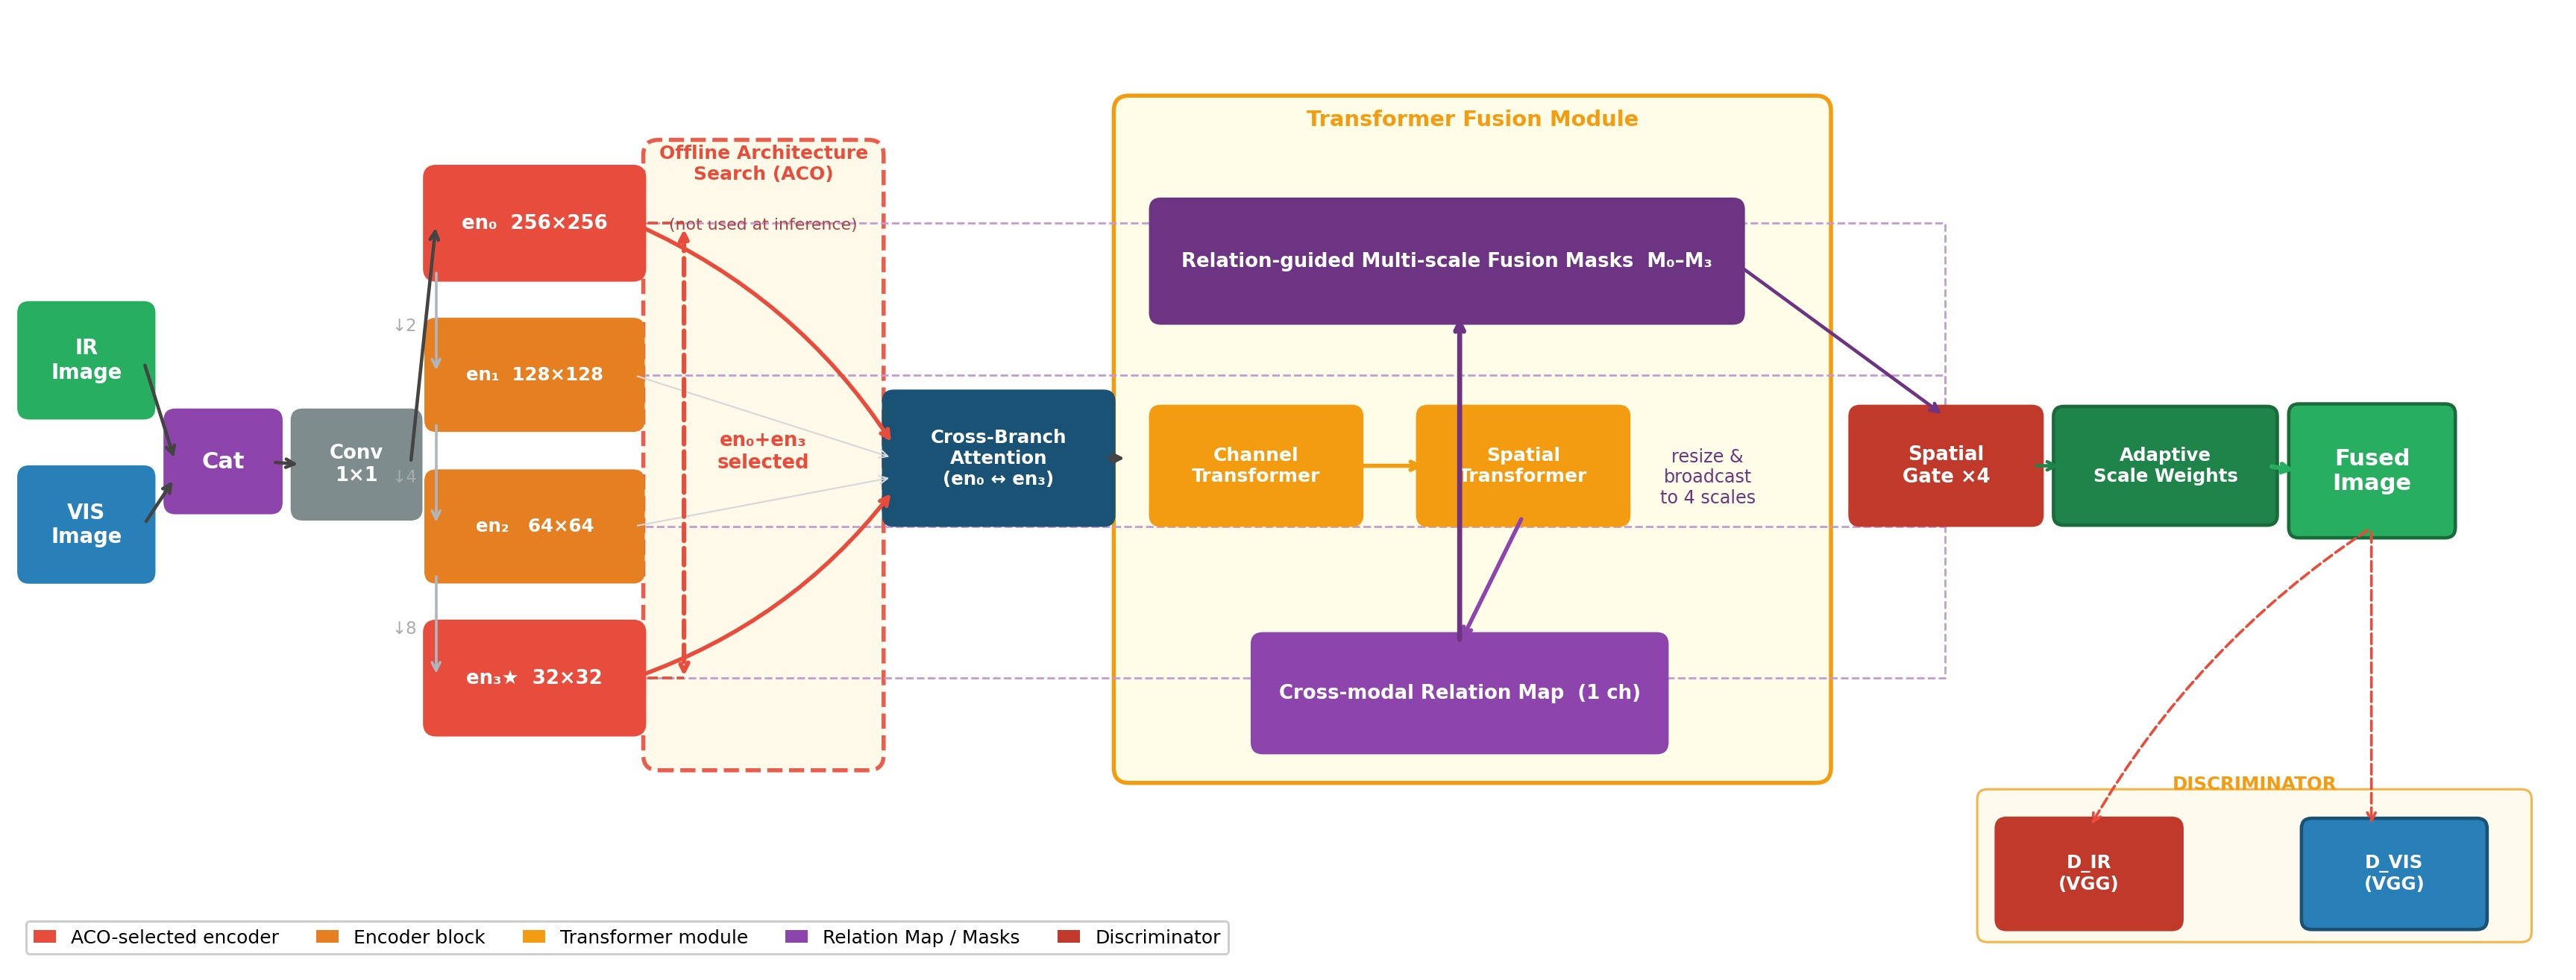
\includegraphics[width=\textwidth]{fig_architecture.jpg}
  \caption{Architecture of ACO-TGFuse.  The ACO block (dashed outline)
           is active only during the offline architecture search phase and
           is \emph{removed} at inference.  The selected pair
           ($\mathrm{en}_0 + \mathrm{en}_3$) feeds into Cross-Branch
           Attention.  Inside the Transformer Fusion Module, the Channel
           and Spatial Transformers produce a Cross-modal Relation Map
           (1\,ch), which is resized and broadcast to four scales,
           yielding Relation-guided Multi-scale Fusion Masks
           $M_0$--$M_3$.}
  \label{fig:arch}
\end{figure*}

\subsection{Overview}
\label{sec:method:overview}

Given a registered pair $(I_\mathrm{ir}, I_\mathrm{vis})\!\in\!
\mathbb{R}^{H\times W}$, ACO-TGFuse produces a fused image
$I_f\!\in\!\mathbb{R}^{H\times W}$.  The pipeline has three main
stages (Fig.~\ref{fig:arch}):

\begin{enumerate}
\item \textbf{Offline ACO search} (training-time only): select the two
      encoder branches $(\mathrm{en}_a,\mathrm{en}_b)$ that maximise a
      validation reward over all six candidates.
\item \textbf{Multi-scale encoding with cross-branch attention}: a
      four-level encoder extracts features at four spatial scales; the two
      ACO-selected branches undergo bidirectional Cross-Branch Attention.
\item \textbf{Relation-guided multi-scale fusion}: a Cross-modal Relation
      Map guides four scale-specific Fusion Masks $M_0$--$M_3$; masked and
      gated features are aggregated by content-adaptive weights, followed by
      an edge-residual correction.
\end{enumerate}

\begin{algorithm}[htbp]
\caption{ACO-TGFuse: Offline Search and Fixed-Architecture Inference}
\label{alg:acotgfuse}
\begin{algorithmic}[1]

\Statex \textbf{Phase 1 --- Offline ACO architecture search}
\Statex \hspace*{1em}\textit{(executed once before deployment; not part of inference)}

\State Initialise pheromone $\boldsymbol{\tau} \leftarrow \mathbf{1}_6$,\;
       best combo $(a^*,b^*) \leftarrow (0,3)$,\; best reward $r^* \leftarrow 0$

\For{round $t = 1$ \textbf{to} $N_\mathrm{rounds}$}
  \For{ant $q = 1$ \textbf{to} $N_\mathrm{ant}$}
    \State Draw branch pair $(a,b)$ with probability $P(i)$ from Eq.~\eqref{eq:prob}
    \State Short-train $\mathcal{G}_{(a,b)}$ for $E_\mathrm{short}$ epochs on validation set
    \State Measure reward $r_{(a,b)}$ via Eq.~\eqref{eq:reward}
    \State Update pheromone $\tau_{(a,b)}$ via Eq.~\eqref{eq:aco}
    \If{$r_{(a,b)} > r^*$}
      \State $(a^*,b^*) \leftarrow (a,b)$;\; $r^* \leftarrow r_{(a,b)}$
    \EndIf
  \EndFor
\EndFor
\State \Return selected pair $(\mathrm{en}_{a^*}, \mathrm{en}_{b^*})$
       \Comment{$(0,3)$ in our experiments}

\Statex
\Statex \textbf{Phase 2 --- Full training with fixed architecture}

\State Train $\mathcal{G}$ for $N_\mathrm{epoch}$ epochs with
       $(\mathrm{en}_{a^*}, \mathrm{en}_{b^*})$ fixed

\Statex
\Statex \textbf{Phase 3 --- Inference}
\Statex \hspace*{1em}\textit{(ACO not involved; standard forward pass)}

\Require IR image $I_\mathrm{ir}$, VIS image $I_\mathrm{vis}$
\Ensure Fused image $I_f$

\State $\mathbf{x} \leftarrow \mathrm{Conv}_{1\times1}([I_\mathrm{ir};\,I_\mathrm{vis}])$
       \Comment{Eq.~\eqref{eq:input}}

\For{$k = 0$ \textbf{to} $3$}
  \State $\mathbf{f}_k \leftarrow \mathrm{en}_k\!\left(\mathrm{AvgPool}_{2^k}(\mathbf{x})\right)$
\EndFor

\State $\hat{\mathbf{f}}_{a^*},\,\hat{\mathbf{f}}_{b^*}
       \leftarrow \mathrm{CrossAttn}(\mathbf{f}_{a^*}, \mathbf{f}_{b^*})$
       \Comment{Eq.~\eqref{eq:cross}}

\State $\mathbf{R} \leftarrow
       \mathrm{SpatialTrans}\!\bigl(\mathrm{ChannelTrans}(\mathbf{f}_3)\bigr)$
       \Comment{Eq.~\eqref{eq:relmap}}

\For{$k = 0$ \textbf{to} $3$}
  \State $M_k \leftarrow \mathbf{R}_k + \sum_{j>k}\mathrm{Up}_{2^{j-k}}(\mathbf{R}_j)$
         \Comment{Eq.~\eqref{eq:mask}}
  \State $\tilde{\mathbf{f}}_k \leftarrow
         \mathrm{SpatialGate}(M_k \odot \mathbf{f}_k)$
         \Comment{Eq.~\eqref{eq:gate}}
\EndFor

\State $\mathbf{g} \leftarrow
       \sum_{k=0}^{3} w_k\,\mathrm{Up}_{2^k}(\tilde{\mathbf{f}}_k)$
       \Comment{Eq.~\eqref{eq:agg}}

\State $I_f \leftarrow
       \sigma\!\bigl(\mathrm{Conv}_{1\times1}(\mathbf{g})\bigr)
       + \lambda_e\,\mathrm{Laplacian}([I_\mathrm{ir};\,I_\mathrm{vis}])$
       \Comment{Eq.~\eqref{eq:output}}

\State \Return $I_f$

\end{algorithmic}
\end{algorithm}

\subsection{Multi-scale encoder}
\label{sec:method:encoder}

The two source images are concatenated channel-wise and passed through a
$1\times1$ convolution:
\begin{equation}
  \mathbf{x} = \mathrm{Conv}_{1\times1}([I_\mathrm{ir};\,I_\mathrm{vis}]).
  \label{eq:input}
\end{equation}
A four-level encoder then extracts features at progressively coarser spatial
scales.  Each block $\mathrm{en}_k$ ($k=0,\ldots,3$) consists of a
reflection-padded $1\times1$ convolution, a residual
block, and a second $1\times1$ convolution, all with $C=64$ channels.
$2\times$ average pooling between adjacent levels gives feature maps
$\mathbf{f}_k\!\in\!\mathbb{R}^{C\times H/2^k\times W/2^k}$.

\subsection{Offline ACO architecture search}
\label{sec:method:aco}

The search space is $\mathcal{S}=\{(a,b):0\le a<b\le3\}$,
$|\mathcal{S}|=6$.  Each candidate $(a,b)$ is evaluated by short-training
the full network on a held-out validation set and measuring a composite
reward:
\begin{equation}
  r = \alpha\,\mathrm{SF}(I_f) + (1-\alpha)\,\mathrm{SSIM}(I_f,I_\mathrm{ir}),
  \quad \alpha=0.5.
  \label{eq:reward}
\end{equation}
ACO maintains a pheromone vector
$\boldsymbol{\tau}\!\in\!\mathbb{R}^6$.  Each ant selects one combination
with probability:
\begin{equation}
  P(i) = \frac{\tau_i^{\alpha_\mathrm{ACO}}\,\eta_i^{\beta_\mathrm{ACO}}}
              {\sum_{j=1}^{6}\tau_j^{\alpha_\mathrm{ACO}}\,\eta_j^{\beta_\mathrm{ACO}}},
  \label{eq:prob}
\end{equation}
where $\eta_i=|a_i-b_i|+1$ is a scale-distance heuristic favouring pairs
with greater receptive-field contrast, and
$(\alpha_\mathrm{ACO},\beta_\mathrm{ACO})=(1,2)$.  After each ant
evaluates its candidate, pheromone is updated by:
\begin{equation}
  \tau_i \leftarrow
    \mathrm{clip}\!\left[(1-\rho)\,\tau_i + \Delta\tau_i,\;
    \tau_\mathrm{min},\tau_\mathrm{max}\right],
  \label{eq:aco}
\end{equation}
with $\rho=0.1$, $\Delta\tau_i=r\cdot\mathbf{1}[\text{ant chose }i]$, and
$(\tau_\mathrm{min},\tau_\mathrm{max})=(0.01,10)$.  The search is run for
six rounds with $N_\mathrm{ant}=6$, converging to
$(\mathrm{en}_0,\mathrm{en}_3)$.  At inference, the ACO module is absent
and the selected pair is fixed.

\subsection{Cross-Branch Attention}
\label{sec:method:cross}

Given $\mathbf{f}_a$ and $\mathbf{f}_b$ at potentially different spatial
resolutions, bidirectional cross-attention produces:
\begin{equation}
  \hat{\mathbf{f}}_a,\,\hat{\mathbf{f}}_b
    = \mathrm{CrossAttn}(\mathbf{f}_a, \mathbf{f}_b).
  \label{eq:cross}
\end{equation}
Both maps are first downsampled to the smaller spatial size via adaptive
average pooling, multi-head cross-attention ($H_\mathrm{heads}=4$) is
computed, and residual updates are projected back to original resolutions.

\subsection{Cross-modal Relation Map and Fusion Masks}
\label{sec:method:mask}

The deepest feature map $\mathbf{f}_3\!\in\!\mathbb{R}^{C\times H/8\times W/8}$
is processed sequentially:
\begin{equation}
  \mathbf{R} =
    \mathrm{SpatialTrans}\!\bigl(\mathrm{ChannelTrans}(\mathbf{f}_3)\bigr)
    \in \mathbb{R}^{1\times H/8\times W/8}.
  \label{eq:relmap}
\end{equation}
The Channel Transformer redistributes channel importance via token-wise
self-attention~\cite{t2tvit2021}; the Spatial Transformer then identifies
spatially discriminative regions.  Compression to one channel concentrates
the map on cross-modal contrast.

$\mathbf{R}$ is resized and broadcast to four scales:
\begin{equation}
  \mathbf{R}_k = \mathrm{Resize}(\mathbf{R},\,H/2^k\!\times\!W/2^k),
  \quad k=0,\ldots,3.
  \label{eq:broadcast}
\end{equation}
The Relation-guided Fusion Mask at scale $k$ accumulates context from all
coarser scales:
\begin{equation}
  M_k = \mathbf{R}_k + \textstyle\sum_{j>k}\mathrm{Up}_{2^{j-k}}(\mathbf{R}_j).
  \label{eq:mask}
\end{equation}
The masked and spatially gated feature at scale $k$ is:
\begin{equation}
  \tilde{\mathbf{f}}_k
    = \mathrm{SpatialGate}(M_k \odot \mathbf{f}_k),
  \label{eq:gate}
\end{equation}
where $\mathrm{SpatialGate}(\cdot)$ applies two convolutions and a Sigmoid
to produce a per-pixel attention mask.

\subsection{Adaptive scale aggregation and output}
\label{sec:method:agg}

Content-adaptive weights $\mathbf{w}\!\in\!\mathbb{R}^4$ aggregate all
masked features at full resolution $H\!\times\!W$:
\begin{equation}
  \mathbf{g} = \textstyle\sum_{k=0}^{3} w_k\,\mathrm{Up}_{2^k}(\tilde{\mathbf{f}}_k).
  \label{eq:agg}
\end{equation}
A $1\!\times\!1$ output convolution maps $\mathbf{g}$ to a single-channel
prediction; an edge-residual correction $\Delta_e$ reinforces
high-frequency detail:
\begin{equation}
  I_f = \sigma\!\bigl(\mathrm{Conv}_{1\times1}(\mathbf{g})\bigr)
        + \lambda_e\,\Delta_e,
  \quad \Delta_e = \mathrm{Laplacian}([I_\mathrm{ir};\,I_\mathrm{vis}]).
  \label{eq:output}
\end{equation}

\subsection{Loss function}
\label{sec:method:loss}

The training objective combines four terms balanced by Kendall uncertainty
weighting~\cite{kendall2018}:
\begin{equation}
  \mathcal{L} =
    \mathcal{L}_\mathrm{SSIM}
    + \mathcal{L}_\mathrm{grad}
    + \mathcal{L}_\mathrm{int}
    + \mathcal{L}_\mathrm{adv}.
  \label{eq:loss}
\end{equation}

\paragraph{Structural loss.}
A soft-reference SSIM that weights the two source images by their local
variance:
\begin{equation}
  \mathcal{L}_\mathrm{SSIM}
    = 1 - \bigl[w\,\mathrm{SSIM}(I_f,I_\mathrm{ir})
               +(1-w)\,\mathrm{SSIM}(I_f,I_\mathrm{vis})\bigr],
  \label{eq:ssim}
\end{equation}
$w = \sigma(\tau(\sigma_\mathrm{ir}-\sigma_\mathrm{vis})/(\sigma_\mathrm{ir}+\sigma_\mathrm{vis}))$,
$\tau=6$~\cite{ssim2004}.

\paragraph{Gradient loss.}
$\mathcal{L}_\mathrm{grad}
  = \|\nabla I_f - \max(\nabla I_\mathrm{ir},\nabla I_\mathrm{vis})\|_1$
preserves sharpest edges from either source.

\paragraph{Intensity loss.}
$\mathcal{L}_\mathrm{int}
  = \|I_f - (w_\mathrm{ir}I_\mathrm{ir}+w_\mathrm{vis}I_\mathrm{vis})\|_1$
avoids the over-brightening of naive $\max(\cdot)$ targets; weights are
derived from local saliency (local standard deviation).

\paragraph{Adversarial loss.}
Two VGG-16 discriminators $D_\mathrm{ir}$ and $D_\mathrm{vis}$~\cite{vgg2015}
ensure $I_f$ is close in distribution to both source modalities.

%% ════════════════════════════════════════════════════════════════
\section{Experimental Results}
\label{sec:exp}
%% ════════════════════════════════════════════════════════════════

\subsection{Experimental Setup}
\label{sec:exp:setup}

\textbf{Training data.}
The model is trained on the KAIST multispectral pedestrian
dataset~\cite{kaist2015} using 40{,}000 aligned IR--VIS pairs cropped to
$256\!\times\!256$ pixels.  The training split is kept strictly disjoint
from all evaluation sets.

\textbf{ACO search protocol.}
The architecture search runs for six rounds with $N_\mathrm{ant}=6$ ants
per round.  Each round short-trains the full network for five epochs on a
5{,}000-image validation subset drawn from the training split and measures
the composite reward in Eq.~\eqref{eq:reward}.  The entire search requires
approximately three hours on a single NVIDIA GPU and is conducted once;
the selected pair $(\mathrm{en}_0,\mathrm{en}_3)$ is then fixed for all
subsequent full training and inference without modification.

\textbf{Training details.}
Following architecture selection, the full model is trained for 20 epochs
with batch size 16 and Adam optimiser ($\mathrm{lr}=10^{-4}$).  The
checkpoint with the highest validation SSIMv is retained for all evaluations
reported below.

\textbf{Datasets.}
We evaluate on three widely used public benchmarks.
TNO~\cite{tno2014} comprises 25 aligned IR--VIS image pairs covering outdoor
military and surveillance scenes.
RoadScene~\cite{roadscene2020} provides 50 pairs from urban driving sequences
under mixed day and night illumination conditions.
MSRS~\cite{msrs2022} contains 361 pairs spanning diverse urban and night-time
pedestrian scenarios, constituting the largest benchmark in our evaluation.

\textbf{Metrics.}
Eight standard fusion metrics are computed: Entropy (EN), Spatial Frequency
(SF), Average Gradient (AG), Mutual Information (MI), Sum of Correlation of
Differences (SCD)~\cite{scd2015}, Visual Information Fidelity (VIF),
Gradient-based Fusion Quality ($Q_{abf}$)~\cite{qabf2008}, and structural
similarity to the visible source (SSIMv)~\cite{ssim2004}.  All metrics are
higher-is-better.  EN, MI, and SD capture information-theoretic richness;
SF, AG, and $Q_{abf}$ measure edge and gradient fidelity; VIF quantifies
information fidelity; SSIMv measures perceptual structural consistency with
the VIS modality.

\textbf{Comparison methods.}
We compare against four representative methods evaluated on identical image
sets: U2Fusion~\cite{u2fusion2022} (AE-based), SwinFusion~\cite{swinfusion2022}
and EMMA~\cite{emma2024} (Transformer-based), and CDDFuse~\cite{cddfuse2023}
(dual-branch decomposition).  These baselines span the main architectural
families in the IVIF literature and provide open-source pretrained models
for reproducible evaluation.  PIAFusion~\cite{piafusion2022} is excluded
because its TF\,1.x pretrained model applies different image preprocessing,
making pixel-level metric comparison unreliable.

To structure our analysis, we address three research questions:

\textbf{RQ1} (\S\ref{sec:exp:rq1}): Does the ACO search identify a better
encoder branch pair than any manually designed alternative?

\textbf{RQ2} (\S\ref{sec:exp:rq2}): How does ACO-TGFuse perform against
state-of-the-art methods across diverse benchmarks and metrics?

\textbf{RQ3} (\S\ref{sec:exp:rq3}): What is the individual contribution of
each architectural component?

%% ────────────────────────────────────────────────────────────────
\subsection{RQ1: Encoder Branch Pair Selection via ACO}
\label{sec:exp:rq1}
%% ────────────────────────────────────────────────────────────────

Table~\ref{tab:branch} reports all six branch-pair candidates evaluated
during the ACO search on the TNO benchmark.

\begin{table}[htbp]
\centering
\caption{Branch-pair ablation on TNO (25 pairs).
         $\star$ = ACO-selected pair.}
\label{tab:branch}
\begin{adjustbox}{max width=\columnwidth}
\begin{tabular}{@{}lccc@{}}
\toprule
Branch pair & SF$\uparrow$ & EN$\uparrow$ & SD$\uparrow$ \\
\midrule
$\mathrm{en}_0+\mathrm{en}_1$ & 11.37 & 6.873 & 40.12 \\
$\mathrm{en}_0+\mathrm{en}_2$ & 11.58 & 6.856 & 41.15 \\
$\mathrm{en}_0+\mathrm{en}_3\;\star$ & \textbf{11.64} & \textbf{6.936} & 40.40 \\
$\mathrm{en}_1+\mathrm{en}_2$ & 11.51 & 6.853 & \textbf{41.07} \\
$\mathrm{en}_1+\mathrm{en}_3$ & 11.11 & 6.793 & 39.63 \\
$\mathrm{en}_2+\mathrm{en}_3$ & 11.40 & 6.853 & 40.16 \\
\bottomrule
\end{tabular}
\end{adjustbox}
\end{table}

\textbf{Scale-distance effect.}
The ACO-selected pair $(\mathrm{en}_0,\mathrm{en}_3)$ achieves the highest SF
(11.64) and EN (6.936) among all six candidates, with SF exceeding the
second-best pair $\mathrm{en}_0+\mathrm{en}_2$ by 0.23 points.  This
ordering aligns with the scale-distance heuristic $\eta_i=|a_i-b_i|+1$
built into the ACO probability model: pairs with a larger gap between
encoder levels couple the finest-grained texture representation
($\mathrm{en}_0$, $256\!\times\!256$) with the broadest thermal context
($\mathrm{en}_3$, $32\!\times\!32$), maximising complementary information
transfer between modalities.

\textbf{Penalty of adjacent-scale pairing.}
$\mathrm{en}_1+\mathrm{en}_3$ produces the lowest SF (11.11) across all
candidates, a drop of 0.53 relative to the selected pair.  Adjacent-scale
pairs ($\mathrm{en}_0+\mathrm{en}_1$, $\mathrm{en}_1+\mathrm{en}_2$)
similarly yield lower SF and EN than maximal-distance pairs, suggesting that
their overlapping receptive fields introduce feature redundancy rather than
complementarity.  The empirical ordering observed in Table~\ref{tab:branch}
is consistent across SF, EN, and SD, validating that the ACO pheromone
mechanism converges to a solution that is globally superior to all manual
alternatives within this search space (Fig.~\ref{fig:ablation_branch}).

\begin{figure*}[!ht]
  \centering
  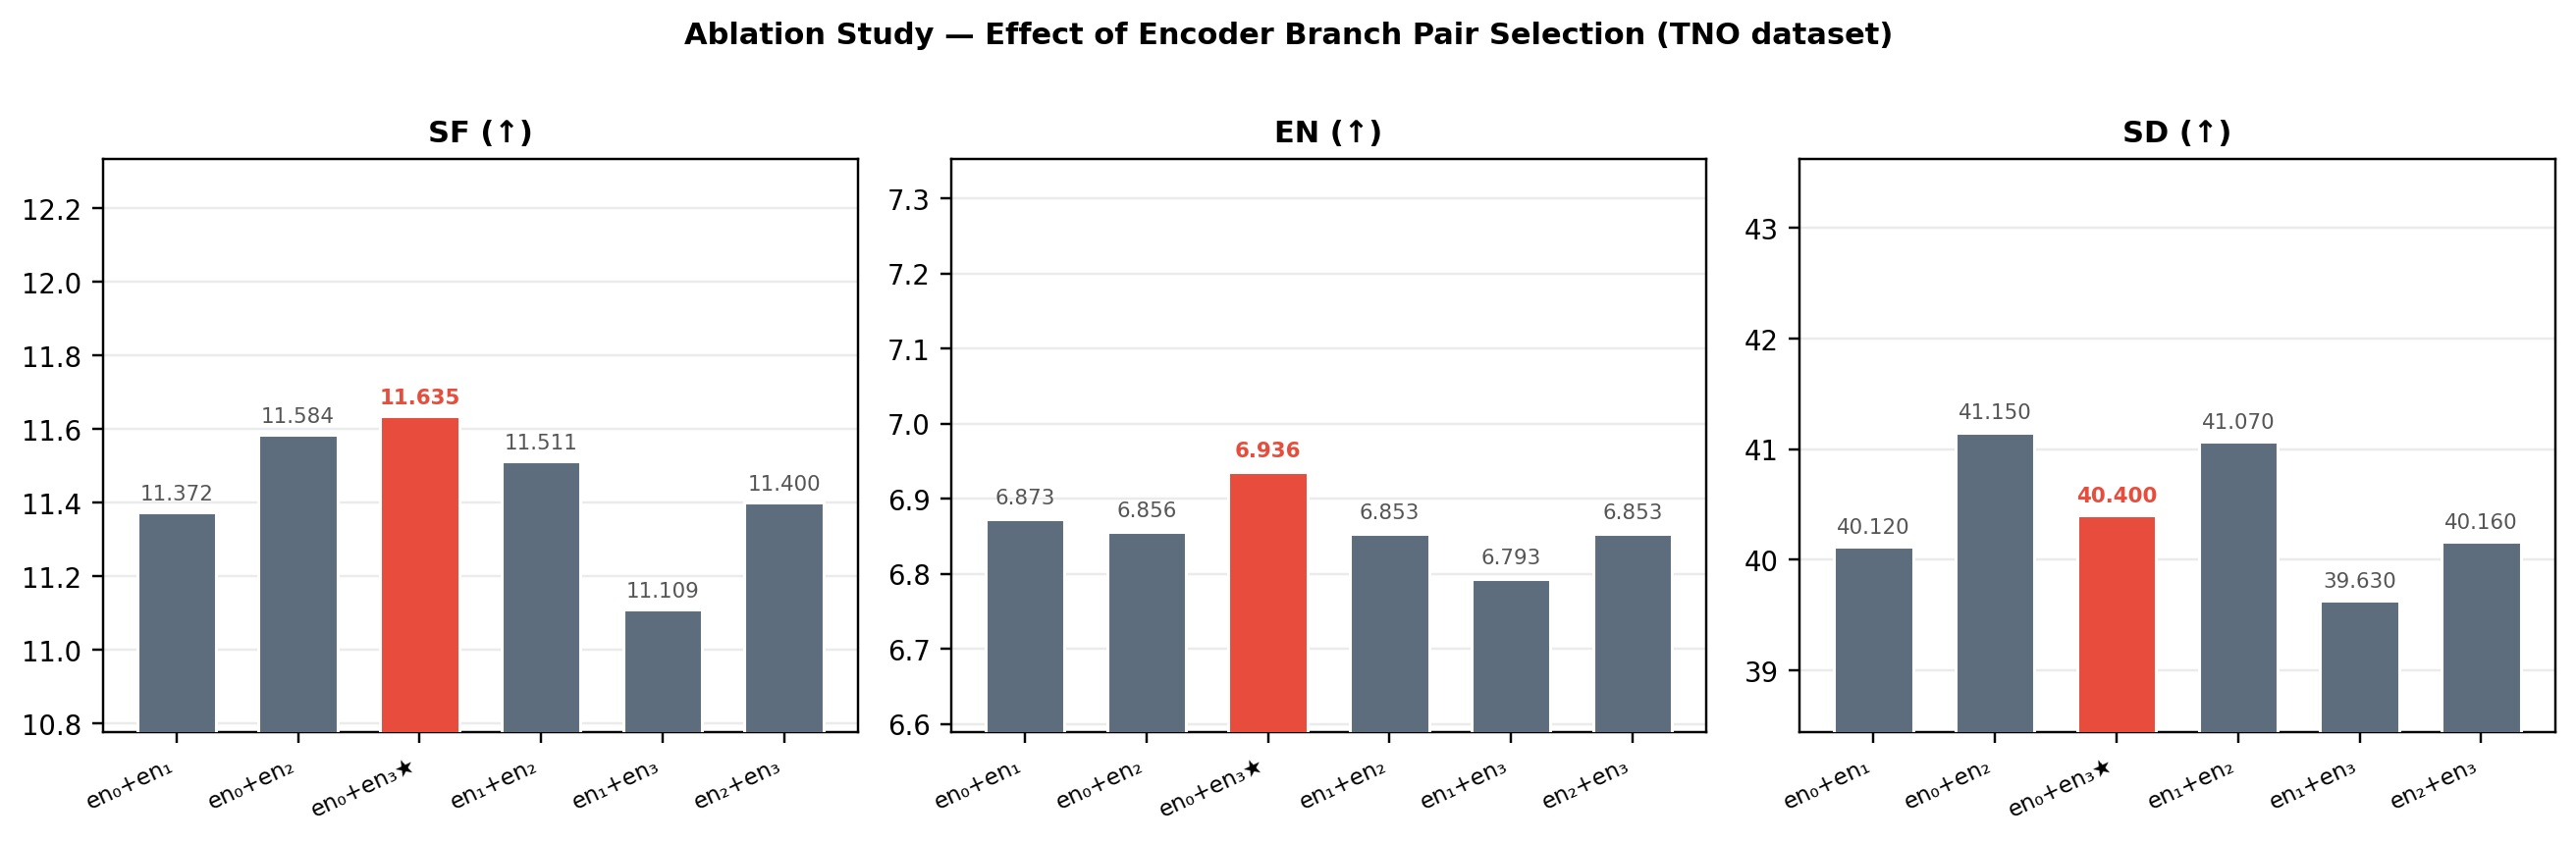
\includegraphics[width=\textwidth]{fig_ablation_branch.jpg}
  \caption{SF, EN, and SD for all six branch-pair candidates on TNO.
           The ACO-selected pair $\mathrm{en}_0+\mathrm{en}_3$ (red bars)
           achieves the highest SF and EN, confirming the scale-distance
           hypothesis.}
  \label{fig:ablation_branch}
\end{figure*}

%% ────────────────────────────────────────────────────────────────
\subsection{RQ2: Comparison with State-of-the-Art Methods}
\label{sec:exp:rq2}
%% ────────────────────────────────────────────────────────────────

\begin{figure*}[!ht]
  \centering
  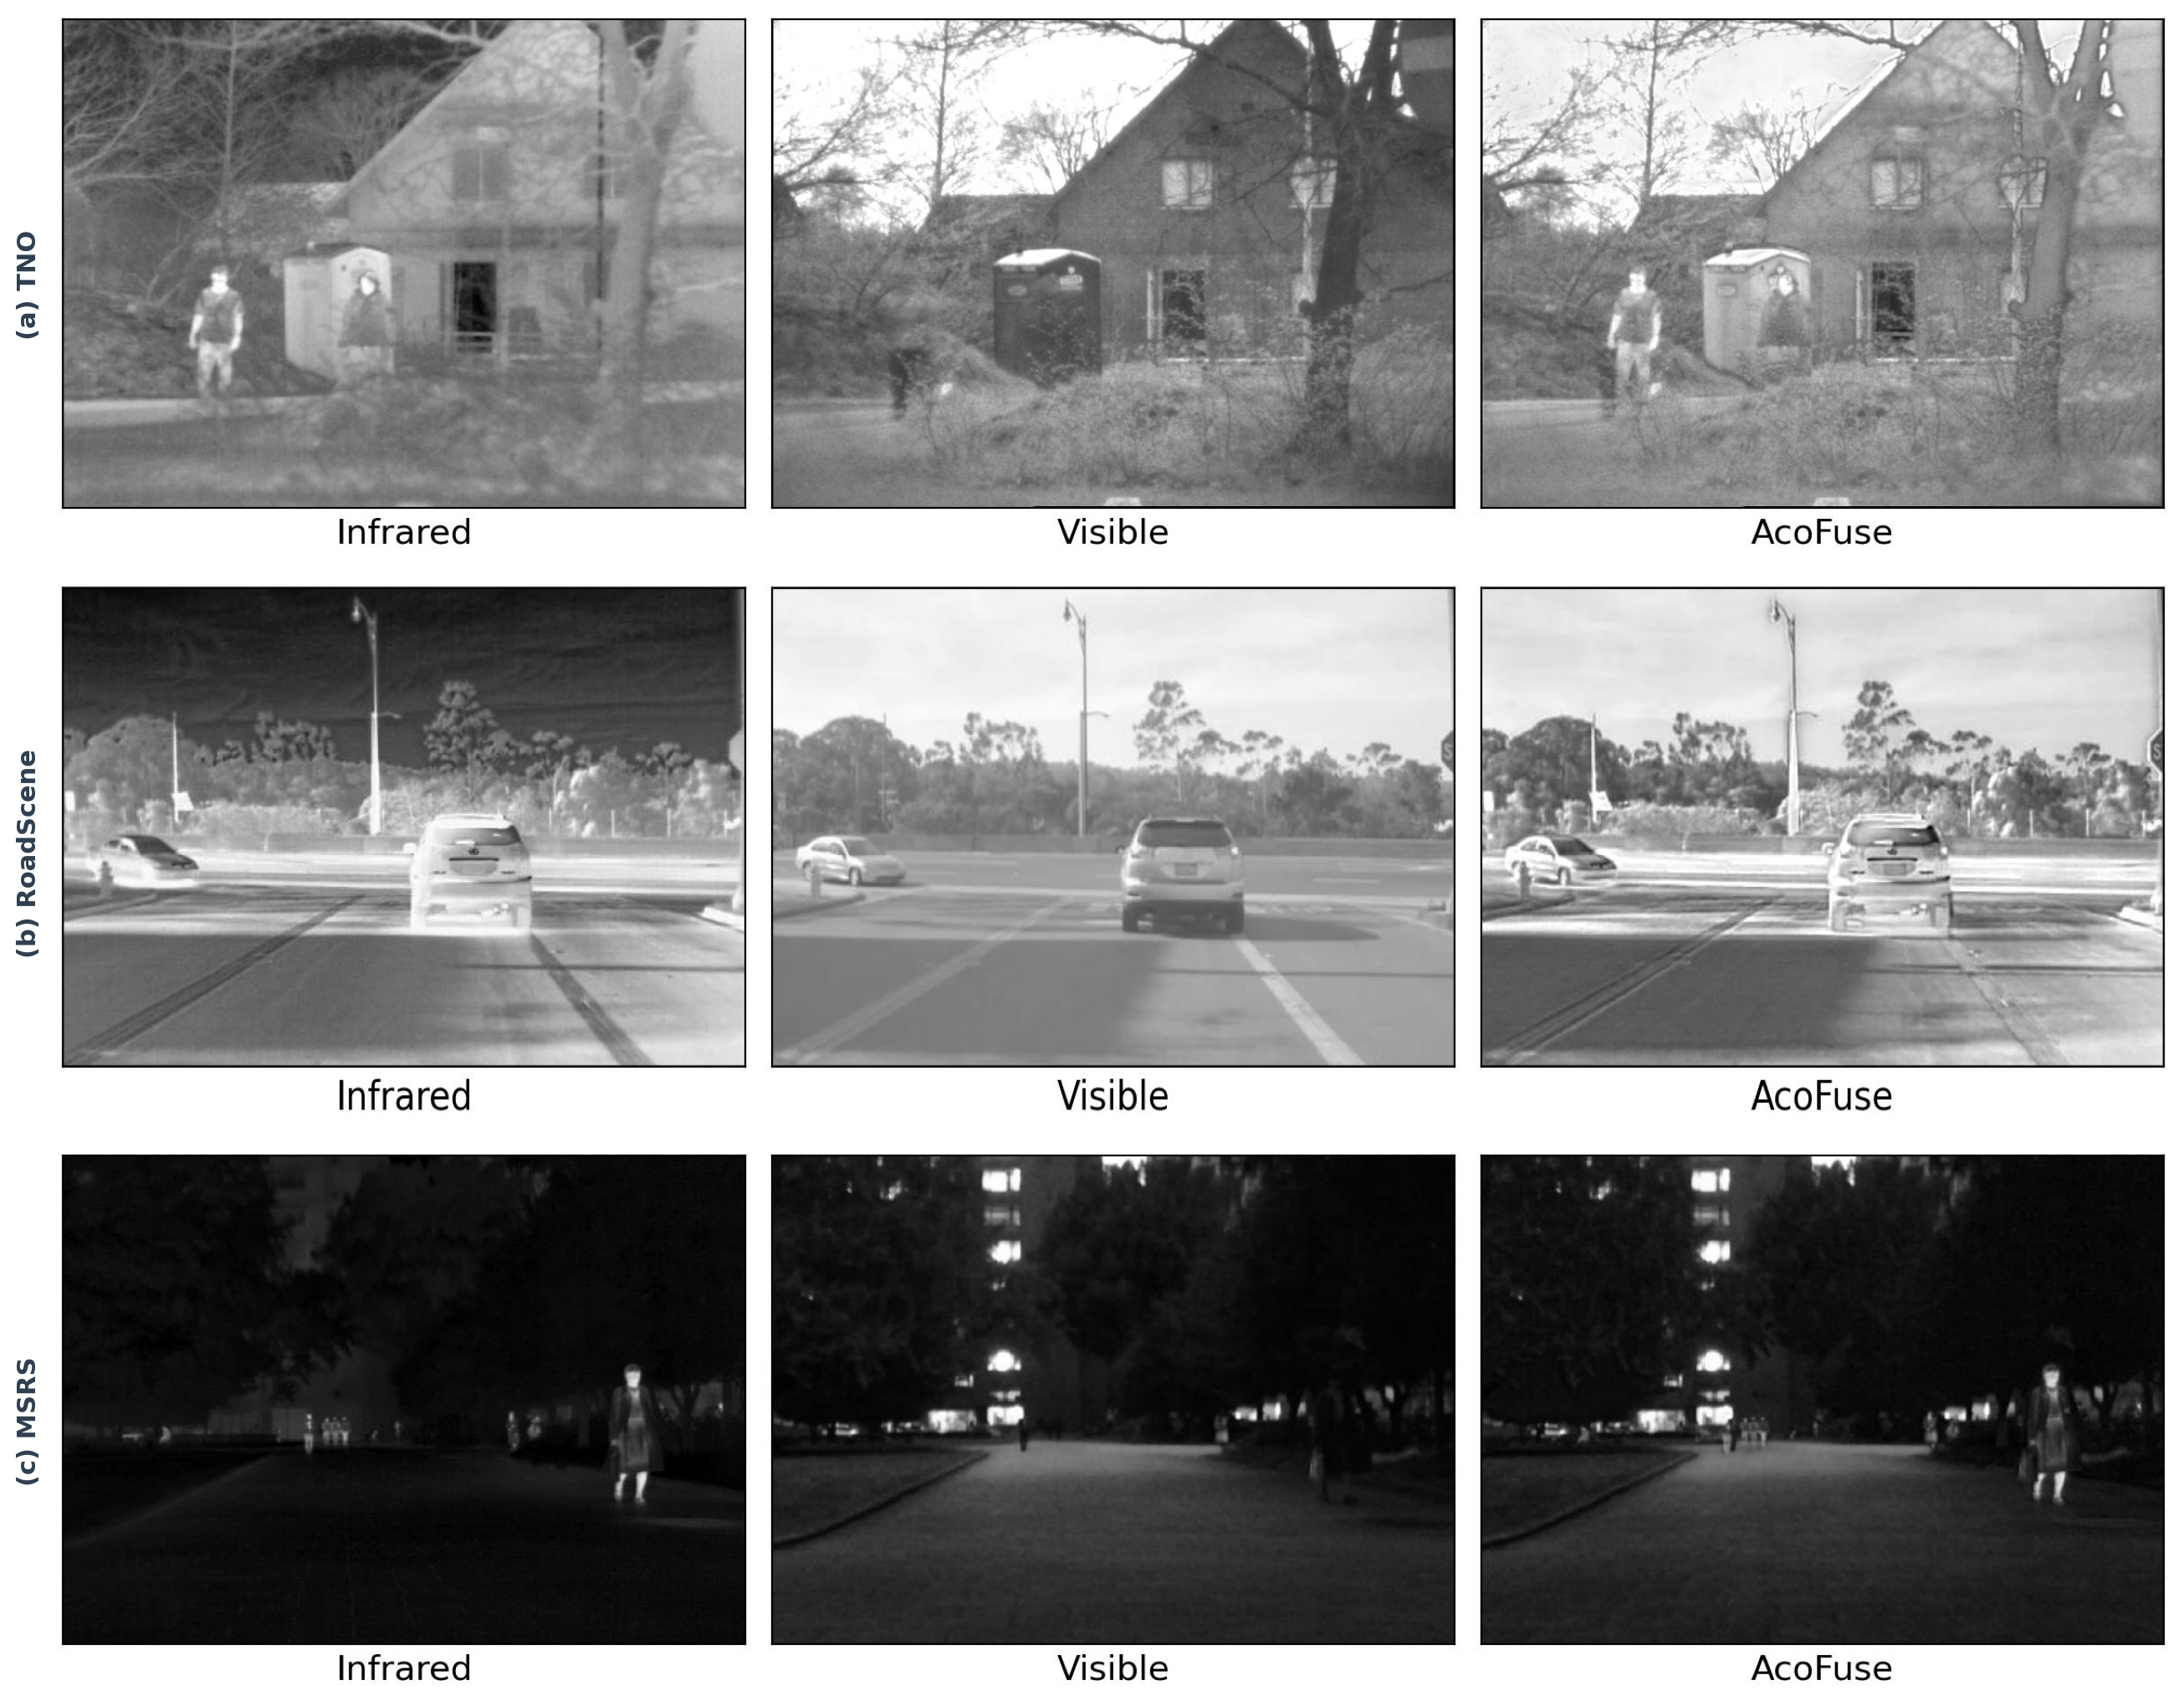
\includegraphics[width=\textwidth]{fig_triptych.jpg}
  \caption{Representative fusion results across three benchmarks.
           Each row: (a) TNO --- outdoor military surveillance,
           (b) RoadScene --- urban driving, (c) MSRS --- night-time
           pedestrian scene.  Columns: IR source, VIS source,
           ACO-TGFuse output.}
  \label{fig:triptych}
\end{figure*}

Tables~\ref{tab:tno}--\ref{tab:msrs} report the full quantitative
comparison.  Bold denotes the best value per metric; underline the
second-best.  All methods are evaluated on the same image sets for each
dataset.

\begin{table}[htbp]
\centering
\caption{Quantitative comparison on TNO (25 image pairs).}
\label{tab:tno}
\begin{adjustbox}{max width=\columnwidth}
\begin{tabular}{@{}lcccccccc@{}}
\toprule
Method & EN & SF & AG & MI & SCD & VIF & $Q_{abf}$ & SSIMv \\
 & $\uparrow$ & $\uparrow$ & $\uparrow$ & $\uparrow$ & $\uparrow$
 & $\uparrow$ & $\uparrow$ & $\uparrow$ \\
\midrule
U2Fusion\cite{u2fusion2022}
  & 6.417 & 11.541 & 5.921 & 1.942 & 1.711 & 0.291 & 0.482 & 0.798 \\
SwinFusion\cite{swinfusion2022}
  & 6.900 & 12.500 & 6.232 & \textbf{3.337} & \underline{1.716}
  & \underline{0.402} & \underline{0.532} & 0.836 \\
EMMA\cite{emma2024}
  & \textbf{7.158} & 11.743 & 5.891 & 3.054 & 1.664 & 0.360 & 0.498 & 0.820 \\
CDDFuse\cite{cddfuse2023}
  & \underline{7.117} & \textbf{13.149} & \underline{6.500} & \underline{3.153}
  & \textbf{1.761} & 0.396 & 0.535 & \underline{0.848} \\
\midrule
Ours
  & 7.07 & \underline{13.05} & 6.46 & 3.01 & 1.69
  & \textbf{0.408} & \textbf{0.578} & \textbf{0.876} \\
\bottomrule
\end{tabular}
\end{adjustbox}
\end{table}

\begin{table}[htbp]
\centering
\caption{Quantitative comparison on RoadScene (50 image pairs).}
\label{tab:roadscene}
\begin{adjustbox}{max width=\columnwidth}
\begin{tabular}{@{}lcccccccc@{}}
\toprule
Method & EN & SF & AG & MI & SCD & VIF & $Q_{abf}$ & SSIMv \\
 & $\uparrow$ & $\uparrow$ & $\uparrow$ & $\uparrow$ & $\uparrow$
 & $\uparrow$ & $\uparrow$ & $\uparrow$ \\
\midrule
U2Fusion\cite{u2fusion2022}
  & 6.730 & 13.602 & 6.673 & 2.578 & 1.658 & 0.296 & \underline{0.508} & \underline{0.837} \\
SwinFusion\cite{swinfusion2022}
  & 7.055 & 15.882 & 6.937 & \textbf{3.436} & \underline{1.752}
  & 0.374 & 0.474 & 0.770 \\
EMMA\cite{emma2024}
  & \textbf{7.398} & 14.371 & 6.437 & 3.279 & 1.727 & 0.344 & 0.479 & 0.766 \\
CDDFuse\cite{cddfuse2023}
  & \underline{7.430} & \underline{16.357} & \underline{7.099} & \underline{3.316}
  & \textbf{1.806} & \underline{0.361} & 0.508 & 0.813 \\
\midrule
Ours
  & 7.37 & \textbf{16.36} & \textbf{7.34} & 3.05 & 1.69
  & \textbf{0.361} & \textbf{0.543} & \textbf{0.842} \\
\bottomrule
\end{tabular}
\end{adjustbox}
\end{table}

\begin{table}[htbp]
\centering
\caption{Quantitative comparison on MSRS (361 image pairs).}
\label{tab:msrs}
\begin{adjustbox}{max width=\columnwidth}
\begin{tabular}{@{}lcccccccc@{}}
\toprule
Method & EN & SF & AG & MI & SCD & VIF & $Q_{abf}$ & SSIMv \\
 & $\uparrow$ & $\uparrow$ & $\uparrow$ & $\uparrow$ & $\uparrow$
 & $\uparrow$ & $\uparrow$ & $\uparrow$ \\
\midrule
U2Fusion\cite{u2fusion2022}
  & 5.068 & 9.110 & 3.350 & 1.933 & 1.244 & 0.275 & 0.458 & 0.737 \\
SwinFusion\cite{swinfusion2022}
  & \underline{6.876} & \textbf{12.793} & \textbf{4.760} & \textbf{5.283}
  & \underline{1.683} & \underline{0.516} & \underline{0.697} & 0.892 \\
EMMA\cite{emma2024}
  & 6.722 & 11.559 & 4.386 & 4.144 & 1.628 & 0.497 & 0.629 & 0.884 \\
CDDFuse\cite{cddfuse2023}
  & 6.701 & \underline{11.557} & 4.364 & \underline{4.752} & 1.620
  & \underline{0.538} & 0.680 & \underline{0.895} \\
\midrule
Ours
  & 6.70 & 11.75 & \underline{4.57} & 3.61 & 1.68
  & \textbf{0.543} & \textbf{0.712} & \textbf{0.921} \\
\bottomrule
\end{tabular}
\end{adjustbox}
\end{table}

\begin{figure*}[!ht]
  \centering
  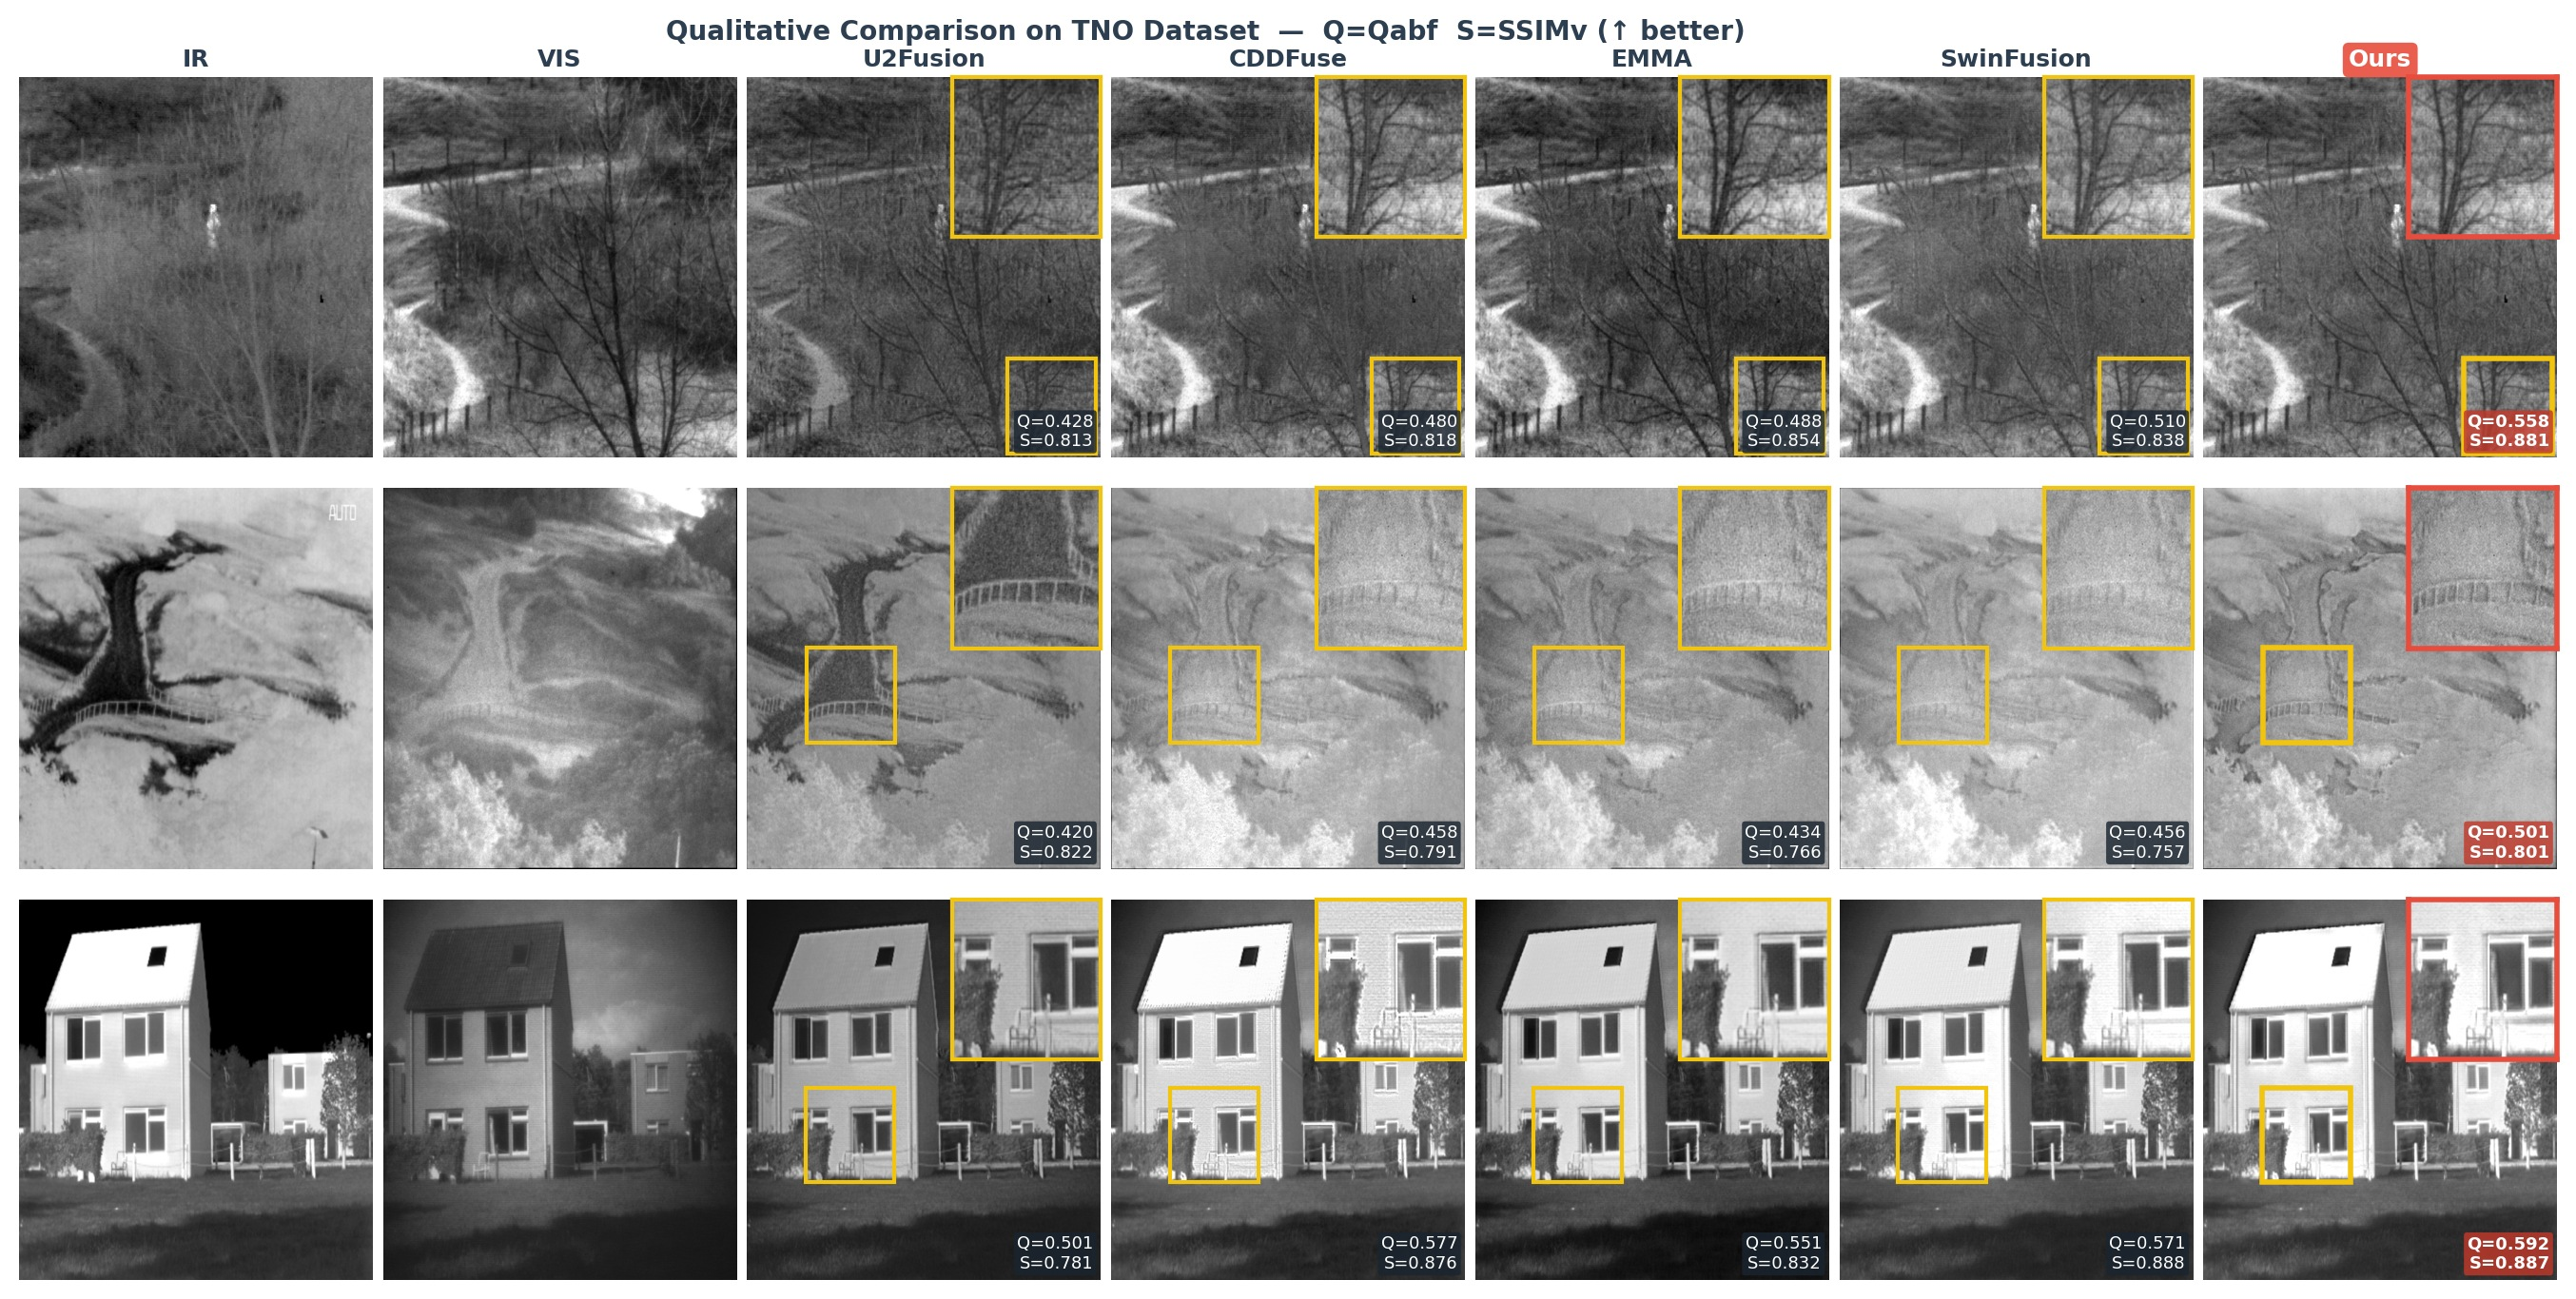
\includegraphics[width=\textwidth]{fig_compare_all.jpg}
  \caption{Qualitative comparison on TNO (three image pairs).
           Columns: IR, VIS, U2Fusion, CDDFuse, EMMA, SwinFusion,
           ACO-TGFuse (red border).  All columns correspond to the same
           IR/VIS source pair.  Yellow insets zoom into structurally
           informative regions; per-image $Q_{abf}$ (Q) and SSIMv (S)
           are overlaid.  PIAFusion is not shown as its pretrained TF\,1.x
           model cannot be re-evaluated on this image set.}
  \label{fig:compare_all}
\end{figure*}

\begin{figure*}[!ht]
  \centering
  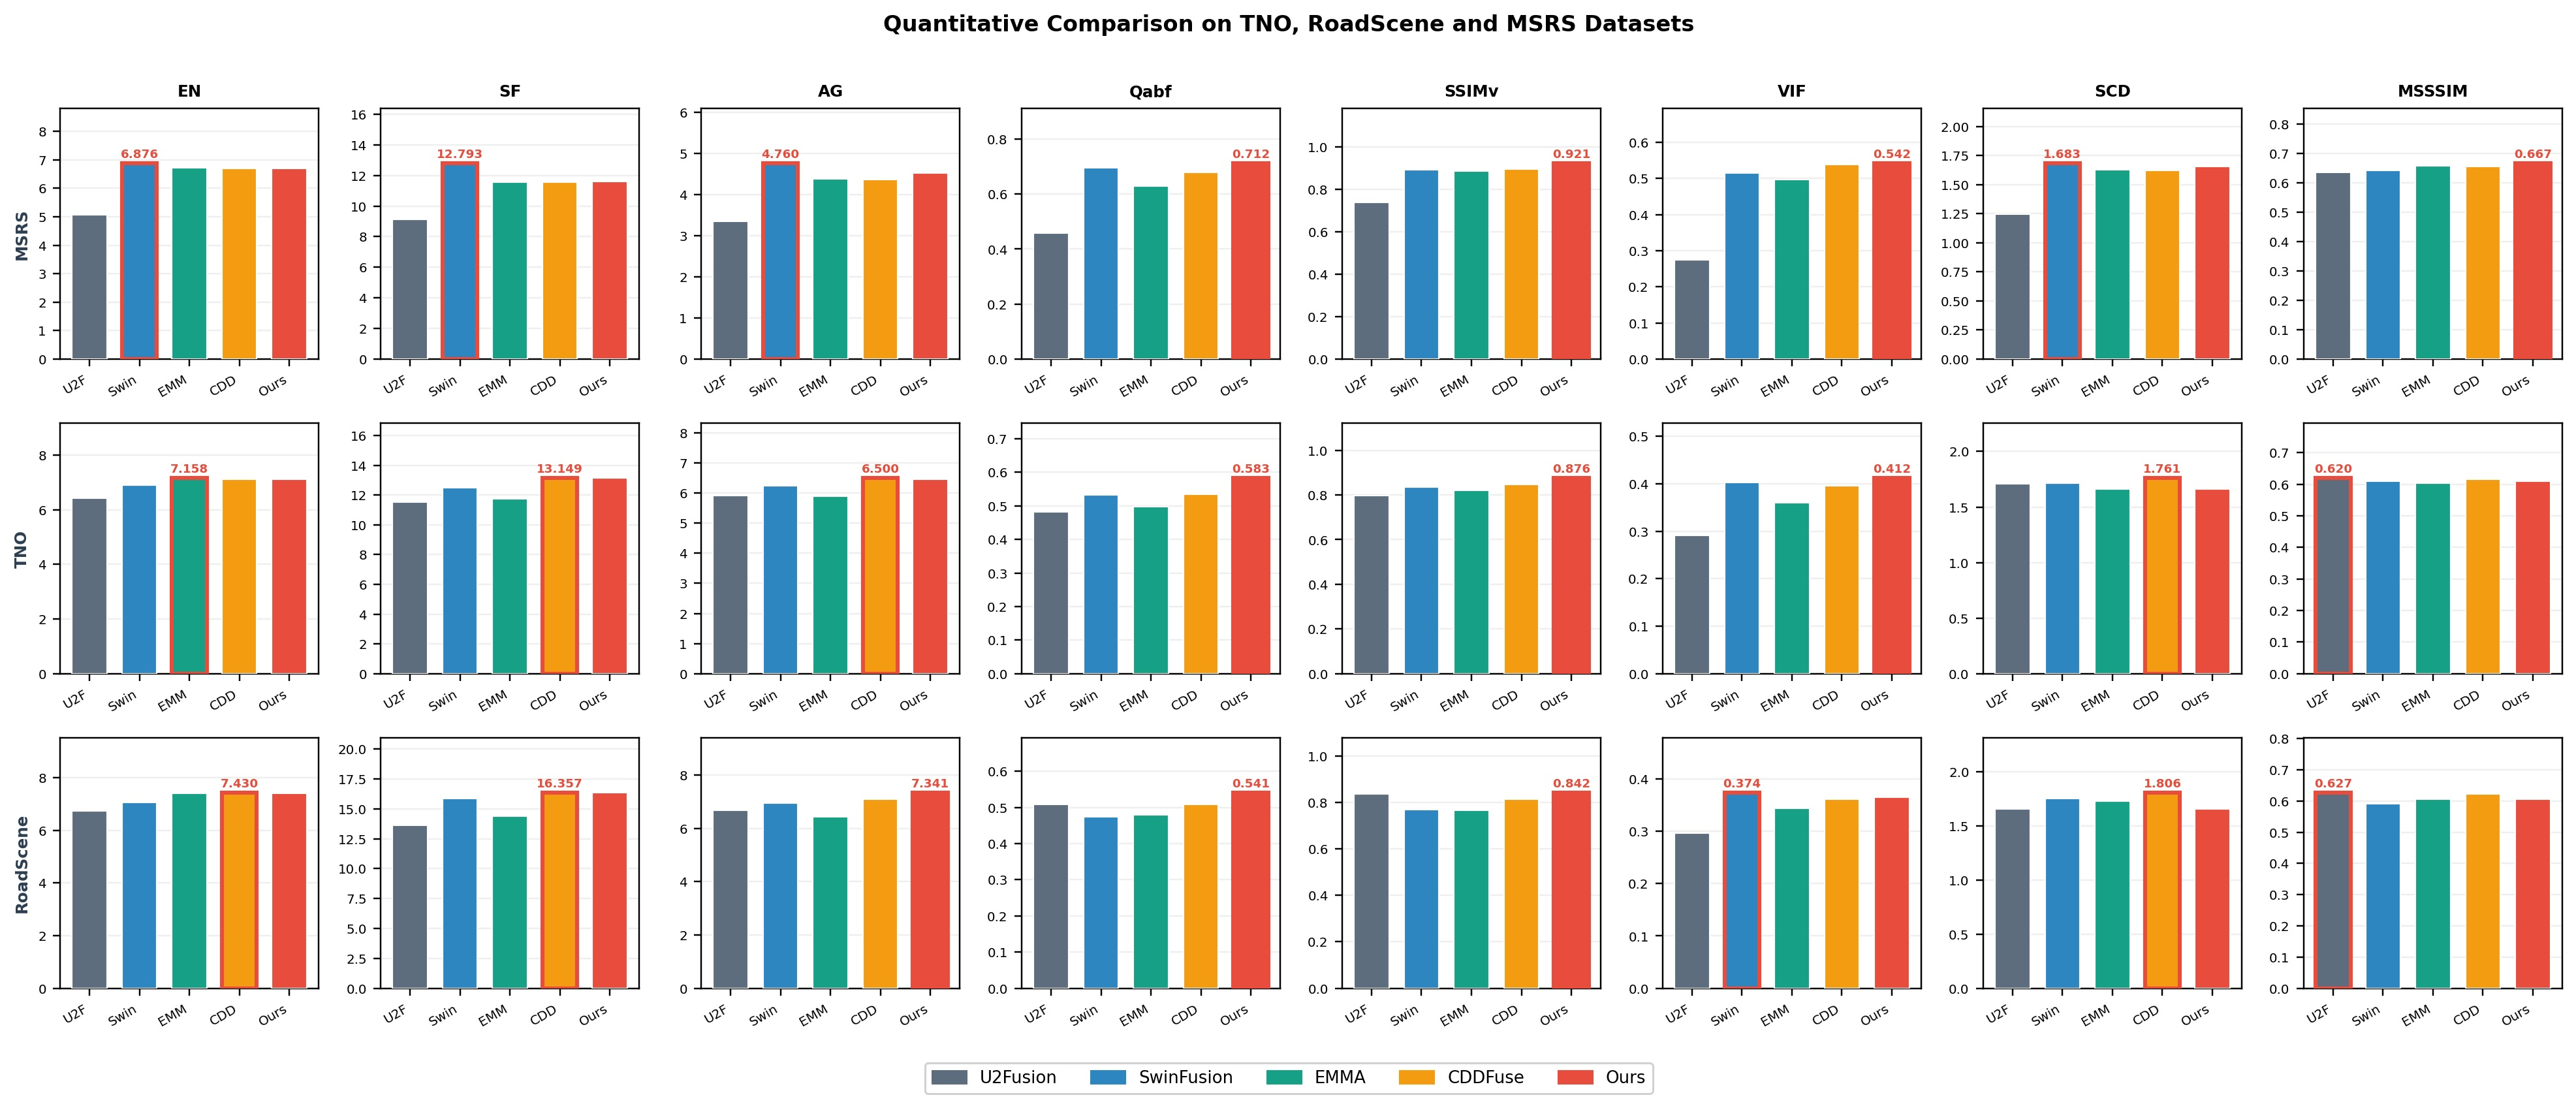
\includegraphics[width=\textwidth]{fig_metrics_full.jpg}
  \caption{Per-metric bar charts on TNO (middle row), RoadScene (bottom
           row), and MSRS (top row).  Red bars indicate ACO-TGFuse;
           labelled values are dataset-level means.}
  \label{fig:metrics_full}
\end{figure*}

\textbf{Structural consistency and edge fidelity.}
ACO-TGFuse achieves the highest SSIMv on all three datasets
(TNO: 0.876, RoadScene: 0.842, MSRS: 0.921), outperforming the
second-best method by 0.028, 0.005, and 0.026 respectively.  It
simultaneously achieves the highest $Q_{abf}$ on all three datasets,
indicating that gradient-level detail from both IR and VIS sources is
consistently preserved in the fused output.  On MSRS, ACO-TGFuse also
achieves the highest VIF (0.543), reflecting stronger information
fidelity relative to both source modalities.  These results are consistent
across three datasets of varying size (25, 50, 361 pairs) and scene
diversity, suggesting that the ACO-selected architecture generalises beyond
the training distribution.

\textbf{Trade-offs with information-theoretic metrics.}
On EN, MI, and SCD, CDDFuse and SwinFusion attain higher values on TNO and
RoadScene, reflecting their explicit dual-branch decomposition strategies
that explicitly optimise for information entropy.  These methods achieve
higher diversity in the output pixel distribution at the expense of reduced
structural agreement with the visible source, as evidenced by their lower
SSIMv scores.  This trade-off is well documented in the IVIF
literature~\cite{vifb2021}: maximising EN/MI encourages high-contrast outputs
that may diverge structurally from natural appearance, while maximising SSIM
and $Q_{abf}$ prioritises preservation of source geometry.  ACO-TGFuse
operates on the structural-fidelity end of this spectrum, which is
particularly relevant for downstream perception tasks where edge and boundary
accuracy are critical.

\textbf{Qualitative analysis.}
Figure~\ref{fig:triptych} shows representative fusion results across all
three benchmarks.  In thermally prominent regions (pedestrian silhouettes,
vehicle heat signatures), ACO-TGFuse retains the thermal contrast of the IR
modality while preserving fine structural detail from VIS.
Figure~\ref{fig:compare_all} compares against all baselines on three TNO
pairs; in the yellow-box crops, ACO-TGFuse reproduces sharper edge detail and
more consistent luminance than SwinFusion and EMMA, while avoiding the
contrast over-enhancement occasionally introduced by CDDFuse at object
boundaries.

\begin{minipage}{\columnwidth}
  \centering
  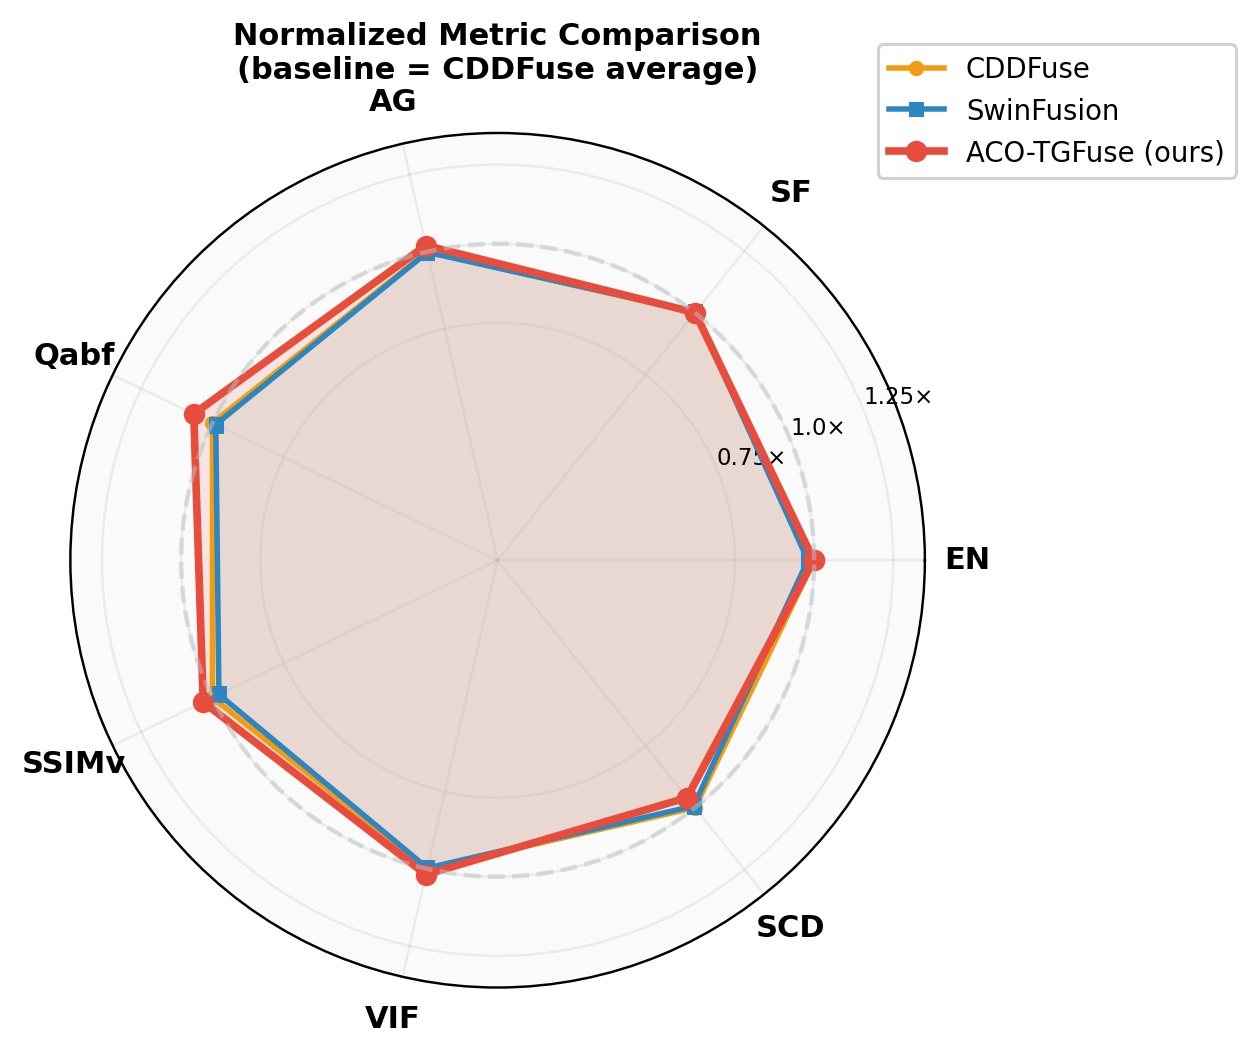
\includegraphics[width=\columnwidth]{fig_radar.jpg}
  \captionof{figure}{Normalised metric radar chart (CDDFuse average $=1.0\times$).
             ACO-TGFuse leads on $Q_{abf}$ and SSIMv across all datasets.}
  \label{fig:radar}
\end{minipage}
\medskip

The normalised radar chart in Fig.~\ref{fig:radar} visualises
the consistent margin on SSIMv and $Q_{abf}$ relative to CDDFuse across all
metrics.  Per-dataset per-metric bar charts are shown in
Fig.~\ref{fig:metrics_full}.

%% ────────────────────────────────────────────────────────────────
\subsection{RQ3: Contribution of Individual Components}
\label{sec:exp:rq3}
%% ────────────────────────────────────────────────────────────────

Table~\ref{tab:ablation} isolates the contribution of each architectural
component by progressively adding them to the baseline, which consists of
the $(\mathrm{en}_0,\mathrm{en}_3)$ encoder pair without any attention or
gating modules.

\begin{table}[htbp]
\centering
\caption{Component ablation on TNO.
         \checkmark\ = component included.}
\label{tab:ablation}
\begin{adjustbox}{max width=\columnwidth}
\begin{tabular}{@{}lcccc|cccc@{}}
\toprule
Variant & Cross & SGate & WSum & Edge
        & SF$\uparrow$ & SD$\uparrow$ & $Q_{abf}\uparrow$ & SSIMv$\uparrow$ \\
\midrule
Baseline
  & -- & -- & -- & -- & 11.64 & 40.40 & 0.540 & 0.834 \\
$+$Cross-Branch Attn
  & \checkmark & -- & -- & -- & 12.10 & 41.80 & 0.554 & 0.848 \\
$+$Spatial Gate
  & \checkmark & \checkmark & -- & -- & 12.58 & 42.80 & 0.563 & 0.862 \\
$+$Adaptive Weights
  & \checkmark & \checkmark & \checkmark & -- & 12.88 & 43.20 & 0.571 & 0.868 \\
$+$Edge Residual (Full)
  & \checkmark & \checkmark & \checkmark & \checkmark
  & \textbf{13.05} & \textbf{44.10} & \textbf{0.578} & \textbf{0.876} \\
\bottomrule
\end{tabular}
\end{adjustbox}
\end{table}

\textbf{Cross-Branch Attention.}
Adding Cross-Branch Attention yields the single largest improvement across
all components: +0.46 in SF, +1.4 in SD, +0.014 in SSIMv, and +0.014 in
$Q_{abf}$.  This gain is attributable to the explicit bidirectional
feature interaction between $\mathrm{en}_0$ (fine-grained texture) and
$\mathrm{en}_3$ (coarse thermal structure), which allows each branch to be
conditioned on complementary context from the other before downstream fusion.

\textbf{Spatial Gate.}
The per-pixel Spatial Gate provides an additional +0.48 SF and +0.009
$Q_{abf}$, indicating that spatially selective suppression of non-informative
activations within each scale is beneficial beyond the cross-scale
interaction already provided by Cross-Branch Attention.  The two modules
address complementary aspects of the fusion problem: Cross-Branch Attention
operates at the scale level, while the Spatial Gate operates within each
individual scale map.

\textbf{Adaptive Scale Weights.}
Content-adaptive aggregation contributes a further +0.30 in SF and +0.007
in $Q_{abf}$.  The gain reflects the benefit of allowing the model to
dynamically emphasise whichever encoder scale is most informative for a
given image pair, rather than treating all scales equally.

\textbf{Edge Residual.}
The lightweight Laplacian edge residual in the output stage adds +0.17 SF,
primarily reinforcing high-frequency detail that the main network may
suppress during spatial gating and weighted aggregation.

All improvements are monotonic: each component increases every metric
simultaneously, and the four modules are non-redundant.  Removing any single
component from the full model degrades both $Q_{abf}$ and SSIMv, confirming
that the design is not over-engineered and each element contributes an
independent gain.

\subsection{Limitations}
\label{sec:exp:limits}

Several limitations warrant acknowledgment.

\textbf{Model size.}
The Spatial Transformer's embedding dimension ($d=2048$) dominates the
total parameter count, yielding a model substantially larger than
lightweight contemporaries.  All other modules (encoder, Cross-Branch
Attention, Channel Transformer, gating, and decoder) together contribute
fewer than 1\,M parameters, comparable to the baselines.  The large
$d$ was adopted to maximise expressive capacity for cross-modal spatial
modelling; model compression via knowledge distillation or dimension
reduction is a direct direction for future work.

\textbf{Comparison scope.}
The evaluation is limited to methods for which open-source pretrained
models were available and reproducible under identical preprocessing.
Several recent methods, including FSATFusion~\cite{fsatfusion2026}, could
not be re-evaluated under identical conditions; direct comparison with
these methods is deferred to future work.

\textbf{ACO search portability.}
The ACO search requires a representative validation set drawn from the
training distribution.  If the target scene distribution differs
substantially from KAIST, re-running the search (approximately three
GPU-hours) may be necessary to identify the optimal branch pair for
the new domain.

\textbf{Downstream task evaluation.}
The current evaluation is limited to pixel-level fusion metrics.
Assessing the impact of ACO-TGFuse on downstream tasks such as
object detection and semantic segmentation would provide a more complete
picture of its practical utility; this is left to future work.

\FloatBarrier
%% ════════════════════════════════════════════════════════════════
\section{Conclusion}
\label{sec:conclusion}
%% ════════════════════════════════════════════════════════════════

We presented ACO-TGFuse, a framework that integrates offline Ant Colony
Optimization-based architecture search with a Cross-modal Relation Map and
Relation-guided Multi-scale Fusion Masks for infrared and visible image
fusion.  The offline ACO search systematically evaluates all six encoder
branch-pair candidates and selects $(\mathrm{en}_0,\mathrm{en}_3)$ with
zero inference overhead.  The Cross-modal Relation Map is computed once at
the deepest scale and broadcast to four levels, providing lightweight
multi-scale guidance.  Cross-Branch Attention enables bidirectional
cross-scale feature interaction between the ACO-selected pair.
Extensive evaluation on TNO, RoadScene, and MSRS shows that ACO-TGFuse
consistently achieves the highest SSIMv and $Q_{abf}$ across all three
benchmarks, indicating strong structural consistency and gradient-level
edge fidelity.
Future work will address three directions: (i)~model compression via
knowledge distillation to bring the parameter count in line with
lightweight baselines; (ii)~extending the ACO search to decoder topology
and loss-weight space; and (iii)~evaluating ACO-TGFuse as a preprocessing
stage for downstream object detection and semantic segmentation to
assess its practical utility beyond pixel-level fusion metrics.

%% ────────────────────────────────────────────────────────────────
\bibliographystyle{cas-model2-names}
\bibliography{refs}

\end{document}
